\documentclass[journal, monochrome]{IEEEtran}
\usepackage[utf8]{inputenc}
\usepackage[monochrome]{color}
\usepackage{graphicx}
\usepackage{amsmath}
\usepackage{amssymb}
\usepackage{fancyvrb}
\usepackage{dsfont}
\usepackage{subfigure}
\usepackage{natbib}
\usepackage{moreverb}
\usepackage{url}
\usepackage{listings}
\usepackage{courier}
\usepackage{caption}

\lstloadlanguages{Octave}
\captionsetup[lstlisting]{ singlelinecheck=false, margin=0pt, font={bf,footnotesize}}
\lstset{
  basicstyle=\footnotesize\ttfamily,
  %numbers=left,
  numberstyle=\tiny,
  %stepnumber=2,
  numbersep=5pt,
  tabsize=8,
  extendedchars=true,
  breaklines=true,
  framexleftmargin=17pt,
  framexrightmargin=5pt,
  showstringspaces=false
}

\ifCLASSINFOpdf
\else
\fi
% graphicx was written by David Carlisle and Sebastian Rahtz. It is
% required if you want graphics, photos, etc. graphicx.sty is already
% installed on most LaTeX systems. The latest version and documentation can
% be obtained at: 
% http://www.ctan.org/tex-archive/macros/latex/required/graphics/
% Another good source of documentation is "Using Imported Graphics in
% LaTeX2e" by Keith Reckdahl which can be found as epslatex.ps or
% epslatex.pdf at: http://www.ctan.org/tex-archive/info/
%
% latex, and pdflatex in dvi mode, support graphics in encapsulated
% postscript (.eps) format. pdflatex in pdf mode supports graphics
% in .pdf, .jpeg, .png and .mps (metapost) formats. Users should ensure
% that all non-photo figures use a vector format (.eps, .pdf, .mps) and
% not a bitmapped formats (.jpeg, .png). IEEE frowns on bitmapped formats
% which can result in "jaggedy"/blurry rendering of lines and letters as
% well as large increases in file sizes.
%
% You can find documentation about the pdfTeX application at:
% http://www.tug.org/applications/pdftex





% *** MATH PACKAGES ***
%
%\usepackage[cmex10]{amsmath}
% A popular package from the American Mathematical Society that provides
% many useful and powerful commands for dealing with mathematics. If using
% it, be sure to load this package with the cmex10 option to ensure that
% only type 1 fonts will utilized at all point sizes. Without this option,
% it is possible that some math symbols, particularly those within
% footnotes, will be rendered in bitmap form which will result in a
% document that can not be IEEE Xplore compliant!
%
% Also, note that the amsmath package sets \interdisplaylinepenalty to 10000
% thus preventing page breaks from occurring within multiline equations. Use:
%\interdisplaylinepenalty=2500
% after loading amsmath to restore such page breaks as IEEEtran.cls normally
% does. amsmath.sty is already installed on most LaTeX systems. The latest
% version and documentation can be obtained at:
% http://www.ctan.org/tex-archive/macros/latex/required/amslatex/math/





% *** SPECIALIZED LIST PACKAGES ***
%
%\usepackage{algorithmic}
% algorithmic.sty was written by Peter Williams and Rogerio Brito.
% This package provides an algorithmic environment fo describing algorithms.
% You can use the algorithmic environment in-text or within a figure
% environment to provide for a floating algorithm. Do NOT use the algorithm
% floating environment provided by algorithm.sty (by the same authors) or
% algorithm2e.sty (by Christophe Fiorio) as IEEE does not use dedicated
% algorithm float types and packages that provide these will not provide
% correct IEEE style captions. The latest version and documentation of
% algorithmic.sty can be obtained at:
% http://www.ctan.org/tex-archive/macros/latex/contrib/algorithms/
% There is also a support site at:
% http://algorithms.berlios.de/index.html
% Also of interest may be the (relatively newer and more customizable)
% algorithmicx.sty package by Szasz Janos:
% http://www.ctan.org/tex-archive/macros/latex/contrib/algorithmicx/




% *** ALIGNMENT PACKAGES ***
%
%\usepackage{array}
% Frank Mittelbach's and David Carlisle's array.sty patches and improves
% the standard LaTeX2e array and tabular environments to provide better
% appearance and additional user controls. As the default LaTeX2e table
% generation code is lacking to the point of almost being broken with
% respect to the quality of the end results, all users are strongly
% advised to use an enhanced (at the very least that provided by array.sty)
% set of table tools. array.sty is already installed on most systems. The
% latest version and documentation can be obtained at:
% http://www.ctan.org/tex-archive/macros/latex/required/tools/


%\usepackage{mdwmath}
%\usepackage{mdwtab}
% Also highly recommended is Mark Wooding's extremely powerful MDW tools,
% especially mdwmath.sty and mdwtab.sty which are used to format equations
% and tables, respectively. The MDWtools set is already installed on most
% LaTeX systems. The lastest version and documentation is available at:
% http://www.ctan.org/tex-archive/macros/latex/contrib/mdwtools/


% IEEEtran contains the IEEEeqnarray family of commands that can be used to
% generate multiline equations as well as matrices, tables, etc., of high
% quality.


%\usepackage{eqparbox}
% Also of notable interest is Scott Pakin's eqparbox package for creating
% (automatically sized) equal width boxes - aka "natural width parboxes".
% Available at:
% http://www.ctan.org/tex-archive/macros/latex/contrib/eqparbox/





% *** SUBFIGURE PACKAGES ***
%\usepackage[tight,footnotesize]{subfigure}
% subfigure.sty was written by Steven Douglas Cochran. This package makes it
% easy to put subfigures in your figures. e.g., "Figure 1a and 1b". For IEEE
% work, it is a good idea to load it with the tight package option to reduce
% the amount of white space around the subfigures. subfigure.sty is already
% installed on most LaTeX systems. The latest version and documentation can
% be obtained at:
% http://www.ctan.org/tex-archive/obsolete/macros/latex/contrib/subfigure/
% subfigure.sty has been superceeded by subfig.sty.



%\usepackage[caption=false]{caption}
%\usepackage[font=footnotesize]{subfig}
% subfig.sty, also written by Steven Douglas Cochran, is the modern
% replacement for subfigure.sty. However, subfig.sty requires and
% automatically loads Axel Sommerfeldt's caption.sty which will override
% IEEEtran.cls handling of captions and this will result in nonIEEE style
% figure/table captions. To prevent this problem, be sure and preload
% caption.sty with its "caption=false" package option. This is will preserve
% IEEEtran.cls handing of captions. Version 1.3 (2005/06/28) and later 
% (recommended due to many improvements over 1.2) of subfig.sty supports
% the caption=false option directly:
%\usepackage[caption=false,font=footnotesize]{subfig}
%
% The latest version and documentation can be obtained at:
% http://www.ctan.org/tex-archive/macros/latex/contrib/subfig/
% The latest version and documentation of caption.sty can be obtained at:
% http://www.ctan.org/tex-archive/macros/latex/contrib/caption/




% *** FLOAT PACKAGES ***
%
%\usepackage{fixltx2e}
% fixltx2e, the successor to the earlier fix2col.sty, was written by
% Frank Mittelbach and David Carlisle. This package corrects a few problems
% in the LaTeX2e kernel, the most notable of which is that in current
% LaTeX2e releases, the ordering of single and double column floats is not
% guaranteed to be preserved. Thus, an unpatched LaTeX2e can allow a
% single column figure to be placed prior to an earlier double column
% figure. The latest version and documentation can be found at:
% http://www.ctan.org/tex-archive/macros/latex/base/



%\usepackage{stfloats}
% stfloats.sty was written by Sigitas Tolusis. This package gives LaTeX2e
% the ability to do double column floats at the bottom of the page as well
% as the top. (e.g., "\begin{figure*}[!b]" is not normally possible in
% LaTeX2e). It also provides a command:
%\fnbelowfloat
% to enable the placement of footnotes below bottom floats (the standard
% LaTeX2e kernel puts them above bottom floats). This is an invasive package
% which rewrites many portions of the LaTeX2e float routines. It may not work
% with other packages that modify the LaTeX2e float routines. The latest
% version and documentation can be obtained at:
% http://www.ctan.org/tex-archive/macros/latex/contrib/sttools/
% Documentation is contained in the stfloats.sty comments as well as in the
% presfull.pdf file. Do not use the stfloats baselinefloat ability as IEEE
% does not allow \baselineskip to stretch. Authors submitting work to the
% IEEE should note that IEEE rarely uses double column equations and
% that authors should try to avoid such use. Do not be tempted to use the
% cuted.sty or midfloat.sty packages (also by Sigitas Tolusis) as IEEE does
% not format its papers in such ways.


%\ifCLASSOPTIONcaptionsoff
%  \usepackage[nomarkers]{endfloat}
% \let\MYoriglatexcaption\caption
% \renewcommand{\caption}[2][\relax]{\MYoriglatexcaption[#2]{#2}}
%\fi
% endfloat.sty was written by James Darrell McCauley and Jeff Goldberg.
% This package may be useful when used in conjunction with IEEEtran.cls'
% captionsoff option. Some IEEE journals/societies require that submissions
% have lists of figures/tables at the end of the paper and that
% figures/tables without any captions are placed on a page by themselves at
% the end of the document. If needed, the draftcls IEEEtran class option or
% \CLASSINPUTbaselinestretch interface can be used to increase the line
% spacing as well. Be sure and use the nomarkers option of endfloat to
% prevent endfloat from "marking" where the figures would have been placed
% in the text. The two hack lines of code above are a slight modification of
% that suggested by in the endfloat docs (section 8.3.1) to ensure that
% the full captions always appear in the list of figures/tables - even if
% the user used the short optional argument of \caption[]{}.
% IEEE papers do not typically make use of \caption[]'s optional argument,
% so this should not be an issue. A similar trick can be used to disable
% captions of packages such as subfig.sty that lack options to turn off
% the subcaptions:
% For subfig.sty:
% \let\MYorigsubfloat\subfloat
% \renewcommand{\subfloat}[2][\relax]{\MYorigsubfloat[]{#2}}
% For subfigure.sty:
% \let\MYorigsubfigure\subfigure
% \renewcommand{\subfigure}[2][\relax]{\MYorigsubfigure[]{#2}}
% However, the above trick will not work if both optional arguments of
% the \subfloat/subfig command are used. Furthermore, there needs to be a
% description of each subfigure *somewhere* and endfloat does not add
% subfigure captions to its list of figures. Thus, the best approach is to
% avoid the use of subfigure captions (many IEEE journals avoid them anyway)
% and instead reference/explain all the subfigures within the main caption.
% The latest version of endfloat.sty and its documentation can obtained at:
% http://www.ctan.org/tex-archive/macros/latex/contrib/endfloat/
%
% The IEEEtran \ifCLASSOPTIONcaptionsoff conditional can also be used
% later in the document, say, to conditionally put the References on a 
% page by themselves.





% *** PDF, URL AND HYPERLINK PACKAGES ***
%
%\usepackage{url}
% url.sty was written by Donald Arseneau. It provides better support for
% handling and breaking URLs. url.sty is already installed on most LaTeX
% systems. The latest version can be obtained at:
% http://www.ctan.org/tex-archive/macros/latex/contrib/misc/
% Read the url.sty source comments for usage information. Basically,
% \url{my_url_here}.





% *** Do not adjust lengths that control margins, column widths, etc. ***
% *** Do not use packages that alter fonts (such as pslatex).         ***
% There should be no need to do such things with IEEEtran.cls V1.6 and later.
% (Unless specifically asked to do so by the journal or conference you plan
% to submit to, of course. )


% correct bad hyphenation here
\hyphenation{op-tical net-works semi-conduc-tor}


\begin{document}
%
% paper title
% can use linebreaks \\ within to get better formatting as desired
\title{Deformación de un cilindro mediante calor}
%
%
% author names and IEEE memberships
% note positions of commas and nonbreaking spaces ( ~ ) LaTeX will not break
% a structure at a ~ so this keeps an author's name from being broken across
% two lines.
% use \thanks{} to gain access to the first footnote area
% a separate \thanks must be used for each paragraph as LaTeX2e's \thanks
% was not built to handle multiple paragraphs
%

\author{\textbf{Autores:} Alejandro Magnorsky, Andrés Mata Suárez, Mariano Merchante \\[5px]
        Instituto Tecnológico de Buenos Aires}
        
% note the % following the last \IEEEmembership and also \thanks - 
% these prevent an unwanted space from occurring between the last author name
% and the end of the author line. i.e., if you had this:
% 
% \author{....lastname \thanks{...} \thanks{...} }
%                     ^------------^------------^----Do not want these spaces!
%
% a space would be appended to the last name and could cause every name on that
% line to be shifted left slightly. This is one of those "LaTeX things". For
% instance, "\textbf{A} \textbf{B}" will typeset as "A B" not "AB". To get
% "AB" then you have to do: "\textbf{A}\textbf{B}"
% \thanks is no different in this regard, so shield the last } of each \thanks
% that ends a line with a % and do not let a space in before the next \thanks.
% Spaces after \IEEEmembership other than the last one are OK (and needed) as
% you are supposed to have spaces between the names. For what it is worth,
% this is a minor point as most people would not even notice if the said evil
% space somehow managed to creep in.



% The paper headers
%\markboth{Template para los informes de SS, 2011}
%{Shell \MakeLowercase{\textit{et al.}}: Bare Demo of IEEEtran.cls for Journals}
% The only time the second header will appear is for the odd numbered pages
% after the title page when using the twoside option.
% 
% *** Note that you probably will NOT want to include the author's ***
% *** name in the headers of peer review papers.                   ***
% You can use \ifCLASSOPTIONpeerreview for conditional compilation here if
% you desire.




% If you want to put a publisher's ID mark on the page you can do it like
% this:
%\IEEEpubid{0000--0000/00\$00.00~\copyright~2007 IEEE}
% Remember, if you use this you must call \IEEEpubidadjcol in the second
% column for its text to clear the IEEEpubid mark.



% use for special paper notices
%\IEEEspecialpapernotice{(Invited Paper)}












% make the title area
\maketitle

\renewcommand{\abstractname}{Resumen}


\renewcommand{\IEEEkeywordsname}{Palabras clave}
\renewcommand{\refname}{Referencias}
\renewcommand{\tablename}{Tabla}

\begin{abstract}
\boldmath

\end{abstract}
% IEEEtran.cls defaults to using nonbold math in the Abstract.
% This preserves the distinction between vectors and scalars. However,
% if the journal you are submitting to favors bold math in the abstract,
% then you can use LaTeX's standard command \boldmath at the very start
% of the abstract to achieve this. Many IEEE journals frown on math
% in the abstract anyway.

% Note that keywords are not normally used for peerreview papers.
\begin{IEEEkeywords}
Cilindro; Temperatura; Deformación; Diferencias finitas.
\end{IEEEkeywords}






% For peer review papers, you can put extra information on the cover
% page as needed:
% \ifCLASSOPTIONpeerreview
% \begin{center} \bfseries EDICS Category: 3-BBND \end{center}


% \fi
%
% For peerreview papers, this IEEEtran command inserts a page break and
% creates the second title. It will be ignored for other modes.
\IEEEpeerreviewmaketitle
\vspace{1cm}

\section{Introducción}


\vspace{1cm}
%-------------------------------------------------------------------------
\section{Desarrollo}
\label{section:development}
\vspace{0.5cm}
\subsection{Cálculo de la temperatura del cilindro}

La temperatura de un cilindro uniforme puede modelarse como una función $u(r,t)$, donde $r$ es la coordenada radial desde el eje del cilindro y $t$ es el tiempo. Dicha función debe satisfacer la siguiente ecuación diferencial:
\begin{equation}
\frac{\partial^{2} u}{\partial r^{2}} + \frac{1}{r} \frac{\partial u}{\partial r} = \frac{1}{4K} \frac{\partial u}{\partial t}
\label{equation:diff}
\end{equation}
para $\frac{1}{2} < r < 1$, $0< t < 10$ y $K = 0.1$. \\

Las condiciones de contorno, para $0 \leq t \leq 10$, son: \\
\begin{equation}
u(\frac{1}{2}, t) = t
\label{equation:contour1}
\end{equation}
\begin{equation}
u(1, t) = 100 + 40t
\label{equation:contour2}
\end{equation}


Además, la condición inicial, para $\frac{1}{2} \leq r \leq 1$, es:
\begin{equation}
u(r, 0) = 200(r-0.5)
\label{equation:initial}
\end{equation}


El objetivo es, entonces, encontrar una aproximación $v_{k}^{m} \approx u(\frac{1}{2} + k\Delta r, m\Delta t)$, donde $k = 0,1,\dots,n$ 
siendo $n = \frac{1-\frac{1}{2}}{\Delta r}$ y $m = 0,1,\dots,l$ con $l = \frac{10}{\Delta t}$. \\

Para ello, se utilizan las siguientes diferencias finitas:
\begin{itemize}
\item Centradas \\
\begin{equation}
\frac{\partial^{2} u}{\partial r^{2}} = \frac{u(r+\Delta r, t) - 2 u(r,t) + u(r-\Delta r,t)}{\Delta r^{2}} + O(\Delta r^{2})
\end{equation}
\begin{equation}
\frac{\partial u}{\partial r} = \frac{u(r+\Delta r, t) - u(r-\Delta r,t)}{2\Delta r} + O(\Delta r^{2})
\end{equation}
\item Progresiva \\
\begin{equation}
\frac{\partial u}{\partial t} = \frac{u(r, t + \Delta t) - u(r,t)}{\Delta t} + O(\Delta t)
\end{equation}
\end{itemize}

Escribiendo las aproximaciones de las diferencias centradas en la ecuación \eqref{equation:diff}, se obtiene el siguiente esquema: \\
\begin{equation}
\frac{v_{k+1}^{m} - 2v_{k}^{m} + v_{k-1}^{m}}{\Delta r^{2}} + \frac{1}{\frac{1}{2}+k\Delta r} \frac{v_{k+1}^{m}-v_{k-1}^{m}}{2\Delta r} = \frac{1}{4K} \frac{v_{k}^{m+1} - v_{k}^{m}}{\Delta t}
\end{equation}
\begin{equation}
v_{k}^{m+1} = v_{k}^{m} + \frac{4K\Delta t}{\Delta r^{2}} (v_{k+1}^{m} - 2v_{k}^{m} + v_{k-1}^{m}) + \frac{4K\Delta t}{(\frac{1}{2}+k\Delta r)2\Delta r} (v_{k+1}^{m}-v_{k-1}^{m})
\label{equation:diffapprox}
\end{equation}

Las condiciones de contorno y la inicial se deducen de las ecuaciones \eqref{equation:contour1}, \eqref{equation:contour2} y \eqref{equation:initial} :
\begin{equation}
v_{0}^{m} = m\Delta t 
\label{equation:vcontour1}
\end{equation}
\begin{equation}
v_{n}^{m} = 100 + 40m\Delta t 
\label{equation:vcontour2}
\end{equation}
\begin{equation}
v_{k}^{0} = 200(\frac{1}{2}+k\Delta r - 0.5) 
\label{equation:vinitial}
\end{equation}

Las diferencias finitas, utilizadas para construir el esquema de la ecuación \eqref{equation:diffapprox}, tienen errores de $O(\Delta r^{2})$ y $O(\Delta t)$. Por lo tanto, el esquema tiene $O(\Delta r^{2} + \Delta t)$, es decir, orden (2,1). \\

Para analizar la estabilidad, se aplica la Transformada de Fourier de Tiempo Discreto en ambos miembros del esquema de la ecuación \eqref{equation:diffapprox}, junto a las propiedades de desplazamiento en el tiempo y linealidad \citep{mathews}, obteniendo:

\begin{equation}
V_{k}^{m+1} = V_{k}^{m} + \frac{4K\Delta t}{\Delta r^{2}} (V_{k}^{m} e^{i\omega}- 2V_{k}^{m} + V_{k}^{m} e^{-i\omega}) + \frac{4K\Delta t}{r 2\Delta r} (V_{k}^{m} e^{i\omega} - V_{k}^{m} e^{-i\omega})
\end{equation}

Despejando $V_{k}^{m}$:

\begin{equation}
V_{k}^{m+1} = (1 + \frac{4K\Delta t}{\Delta r^{2}} (e^{i\omega} + e^{-i\omega}) - 2\frac{4K\Delta t}{\Delta r^{2}} + \frac{4K\Delta t}{r 2\Delta r} (e^{i\omega} - e^{-i\omega})) V_{k}^{m}
\end{equation}
\begin{equation}
V_{k}^{m+1} = (1 + 2 \frac{4K\Delta t}{\Delta r^{2}}(\cos \omega - 1) + i 2 \frac{4K\Delta t}{r 2\Delta r} \sin \omega) V_{k}^{m}
\end{equation}

Se define $\rho = 1 + 2 \frac{4K\Delta t}{\Delta r^{2}}(\cos \omega - 1) + i 2 \frac{4K\Delta t}{r 2\Delta r} \sin \omega$. Entonces:

\begin{equation}
V_{k}^{m+1} = \rho V_{k}^{m}
\end{equation}
\begin{equation}
V_{k}^{m+1} = \rho^{m+1} V_{k}^{0}
\end{equation}

Por lo tanto, $|\rho| < 1$ para que el método sea estable. Para que eso se cumpla, como mínimo, $|Im(\rho)| < 1$:
\begin{equation}
|2 \frac{4K\Delta t}{r 2\Delta r} \sin \omega| <1 \Rightarrow \frac{4K\Delta t}{r 2\Delta r} < \frac{1}{2} \Rightarrow \Delta t < \frac{r\Delta r}{4 K}
\end{equation}

Considerando los casos en que $r = \frac{1}{2}$ y $r = 1$, se obtiene que el caso más restrictivo es que $\Delta t < \frac{\Delta r}{8 K}$. \\

En la figura \ref{lst:finiteDifferences}, se detalla la implementación de un programa que, dados $\Delta r$ y $\Delta t$, utiliza las condiciones de contorno y la inicial (ecuaciones \eqref{equation:vcontour1}, \eqref{equation:vcontour2} y \eqref{equation:vinitial}) para armar parte de la matriz $v$ que representa a la función $v_{k}^{m}$, donde $k$ es la columna y $m$ es la fila. Para completar el resto, usa el esquema de la ecuación \eqref{equation:diffapprox}. \\



\subsection{Cálculo de la deformación del cilindro}

La deformación del cilindro, $d$, es proporcional a la temperatura media del mismo. Por lo tanto, se calcula como:
\begin{equation}
d(t) = \alpha \int_{\frac{1}{2}}^{1} u(r,t)r dr
\label{equation:deformation}
\end{equation}
donde $\alpha = 10.7$. \\

Para el cálculo de la ecuación \eqref{equation:deformation} se utiliza el método de los trapecios. Se calcula $d(10)$ con parámetros cada vez más chicos, hasta que la diferencia con el resultado anterior sea menor que el 5\%.



\vspace{1cm}
%-------------------------------------------------------------------------
\section{Resultados}
\label{section:results}
\vspace{0.5cm}

Para realizar todos los cálculos se utiliza $\Delta r = 0.1$ y $\Delta t = 0.01$.


\begin{figure}[hbp]
	\centering
	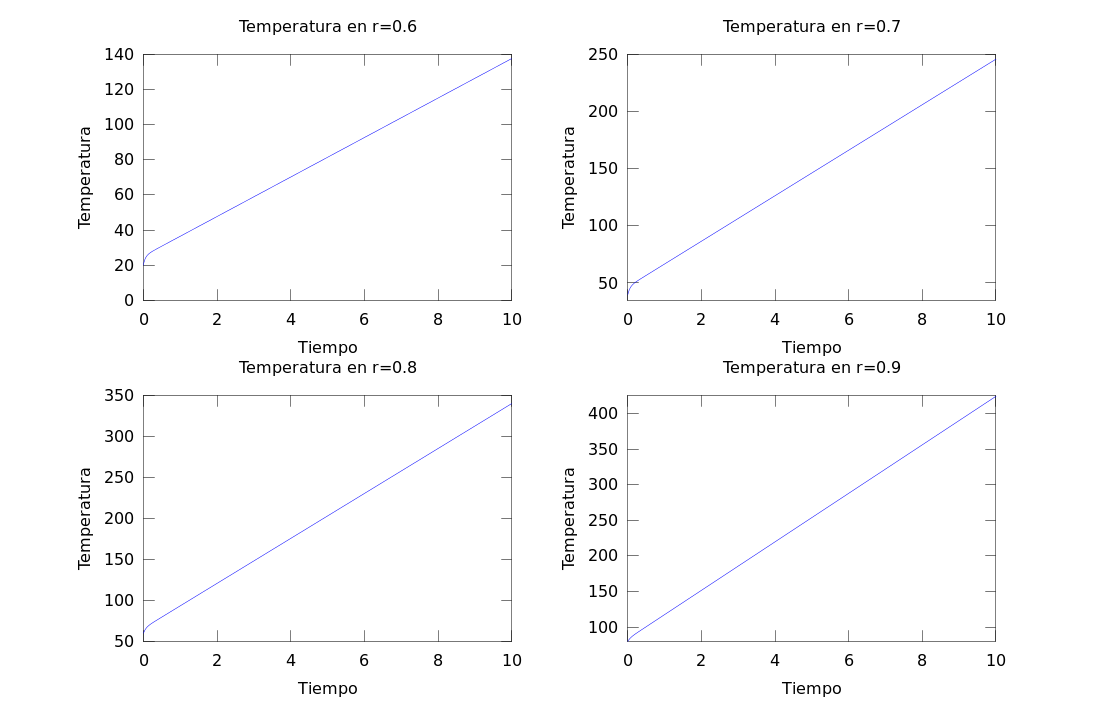
\includegraphics[scale = 0.50]{img/graph_c.png}
	\caption{Temperatura del cilindro para $r = 0.6,0.7,0.8$ y $0.9$}
	\label{figure:histograms}
\end{figure}
\begin{figure}
	\centering
	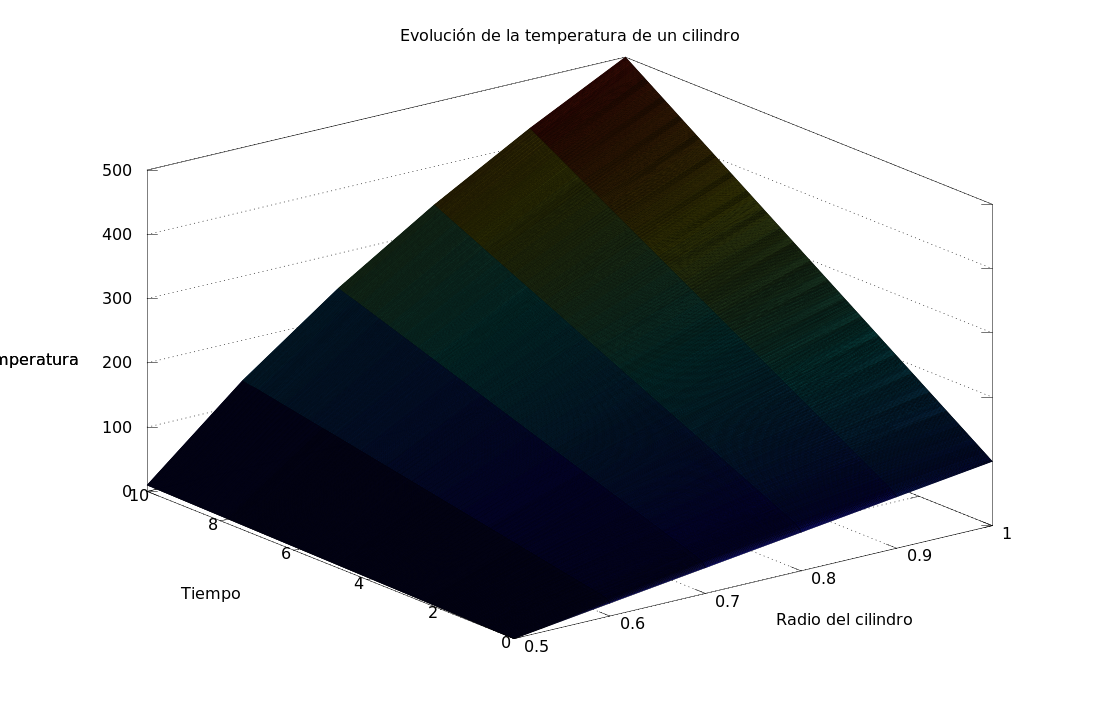
\includegraphics[scale = 0.25]{img/graph_mesh.png}
	\caption{Evolución de la temperatura del cilindro}
	\label{figure:histograms}
\end{figure}
\begin{figure}
	\centering
	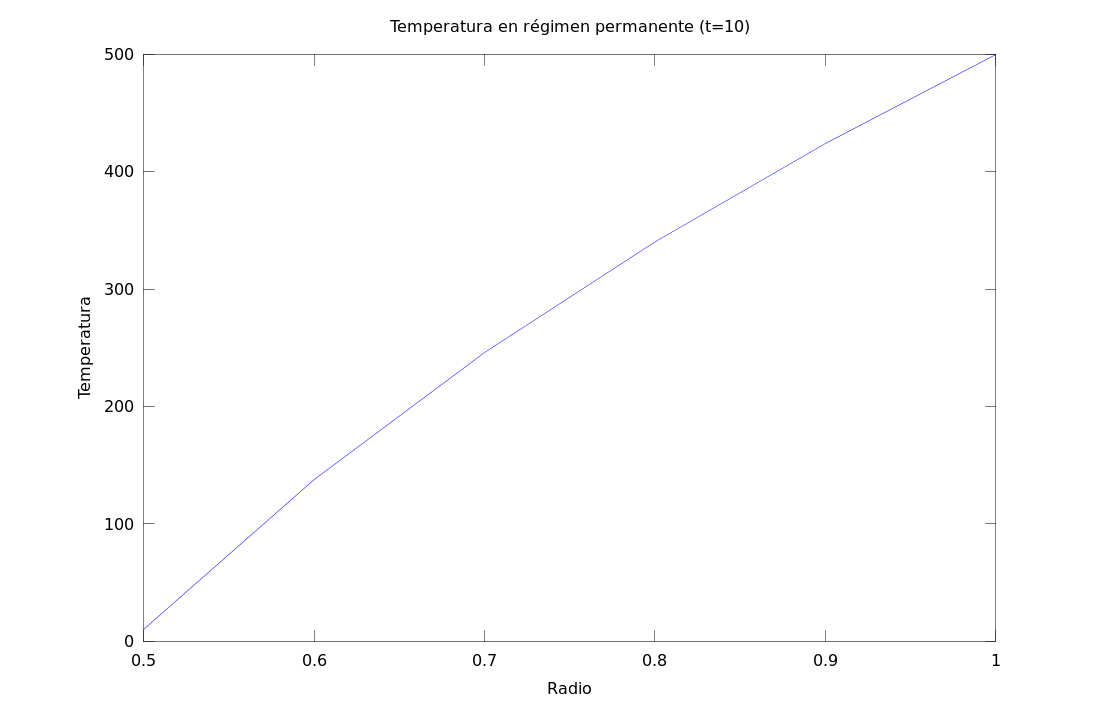
\includegraphics[scale = 0.25]{img/graph_d.png}
	\caption{Temperatura en régimen permamente}
	\label{figure:histograms}
\end{figure}
\begin{figure}
	\centering
	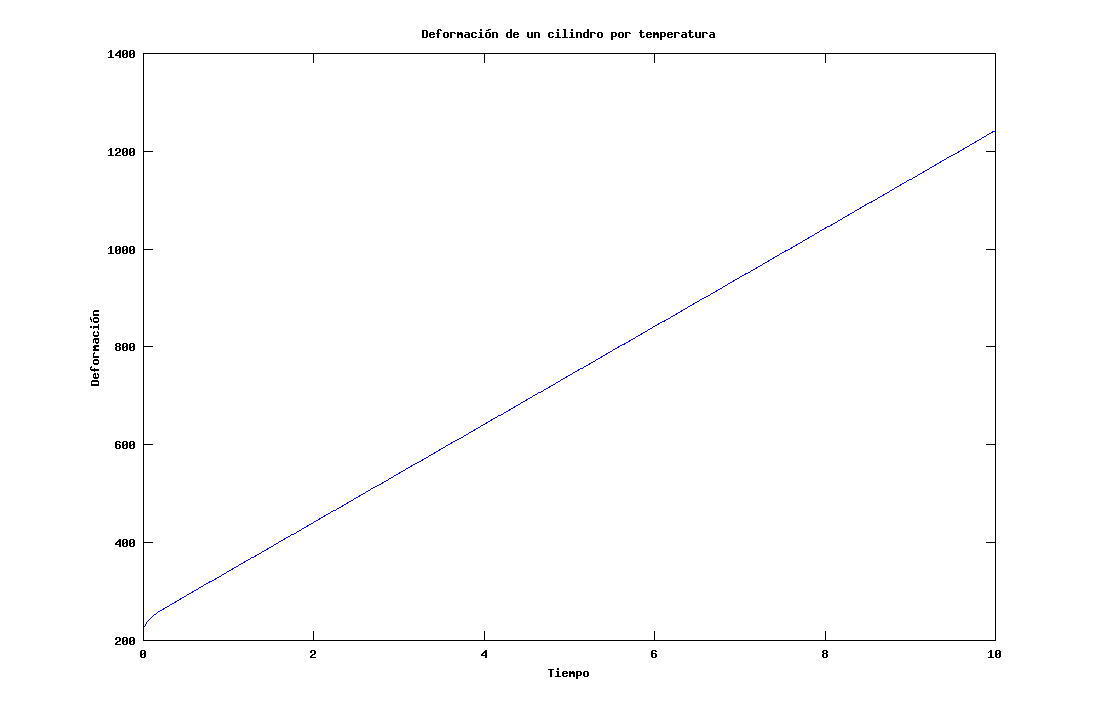
\includegraphics[scale = 0.25]{img/graph_e.png}
	\caption{Deformación del cilindro}
	\label{figure:histograms}
\end{figure}



\vspace{1cm}
\section{Conclusiones}
\label{section:conclusions}
\vspace{0.5cm}



%-------------------------------------------------------------------------

\vspace{1cm}
\begin{thebibliography}{1}
\bibitem[Mathews y Fink(1992)]{mathews}
	Mathews, John H.,
	Fink, Kurtis D.,
	``Numerical Methods Using MATLAB'',
	Prentice Hall,
	1999
	
\end{thebibliography}



%-------------------------------------------------------------------------

\begin{figure}
	\lstinputlisting[label=lst:finiteDifferences,caption=Implementación del cálculo de $v_{k}^{m}$.]{../src/finiteDifferences.m}
\end{figure}

% trigger a \newpage just before the given reference
% number - used to balance the columns on the last page
% adjust value as needed - may need to be readjusted if
% the document is modified later
%\IEEEtriggeratref{8}
% The "triggered" command can be changed if desired:
%\IEEEtriggercmd{\enlargethispage{-5in}}

% references section

% can use a bibliography generated by BibTeX as a .bbl file
% BibTeX documentation can be easily obtained at:
% http://www.ctan.org/tex-archive/biblio/bibtex/contrib/doc/
% The IEEEtran BibTeX style support page is at:
% http://www.michaelshell.org/tex/ieeetran/bibtex/
%\bibliographystyle{IEEEtran}
%\bibliographystyle{authordate}
% argument is your BibTeX string definitions and bibliography database(s)
%\bibliography{IEEEabrv,../bib/paper}
%
% <OR> manually copy in the resultant .bbl file
% set second argument of \begin to the number of references
% (used to reserve space for the reference number labels box)


\end{document}


